\section{Подходы к написанию автоматизированных тестов} 

Процесс тестирования программного обеспечения можно разделить на~две фазы: разработка тестовых сценариев и~запуск тестовых сценариев. 

Разработка тестовых сценариев подразуевает анализ, дизайн и~написание кода. Смысл этой фазы состоит в~том, что бы разработать такое множество тестовых сценариев, которое бы удовлетворяло стандартам качества разрабатываемого программного обеспечения. Понятие <<автоматизированное тестирование>> не включает в себя автоматизацию этой фазы.

Вторая фаза подразумевает инсталяцию программного обеспечения и выполнение тестовых сценариев, разработанных на первой фазе. Запуск тестовых сценариев чаще всего автоматизируется. 


Разработка тестовых сценариев~--- комплексная задача. Сложность ее~состоит в нахождении достаточного набора тестовых сценариев, который удовлетворяет стандартам качества. Одновременно с этим, набор тестов должен быть конечен и выполняться достаточно быстро. Далее будут рассмотренны техники анализа, дизайна и написания тестовых сценариев.


\subsection{Тестирование на основе спецификации} 

Спецификация~--- набор требований к программному обеспечению. Может быть представлена как текстовый файл или UML диаграмма.

Тестирование на основе спецификации~--- подход к разработке минимального набора тестов, которые будут удовлетворять спецификации. Такой подход позволяет абстрагироваться от конкретной реализации системы (тестирование <<черного ящика>>).

Основу этого метода составляет группировка множества входных данных.

 \subsubsection{Группировка множества входных данных}

Пример спецификации. Определение високосного года. На вход программе поступает год в виде числа, программа должна возвращать \texttt{true} если год явлется високосным и \texttt{false} в противном случае. Год високосный, если:

\begin{itemize}
	\item год кратен 4;
	\item год не кратен 100;
	\item исключение: если год кратен 400, то он високосный.
\end{itemize}

Реализация спецификации представленна в листинге 1.4.

\begin{ListingEnv}[!h]% настройки floating аналогичны окружению figure
	\captiondelim{ } % разделитель идентификатора с номером от наименования
	\caption{Определение високосного года}
	% окружение учитывает пробелы и табуляции и применяет их в сответсвии с настройками
	\begin{lstlisting}[language={Java}]
public class LeapYear {
	
	public boolean isLeapYear(int year) {
		if (year % 400 == 0)
		return true;
		if (year % 100 == 0)
		return false;
		
		return year % 4 == 0;
	}
}
	\end{lstlisting}
\end{ListingEnv}%

 Для подбора оптимальных входных данных, нужно разбить программу на классы (группы). Другими словами, нужно разбить множество входных данных следующим образом:
 
 \begin{enumerate}
 	\item каждый класс уникален, т.~е. не существует двух классов, которые приводят к одному и тому же поведению программы;
 	\item поведение программы может быть однозначно интерпритированно как корректное или некорректное.
 \end{enumerate}

Учитывая требования к классам и спецификацию, можно получить следующий набор классов:

 \begin{itemize}
 	\item год кратен 4, но не кратен 100~--- високосный, \texttt{true};
 	\item год кратен 4, кратен 100, кратен 400~--- високосный, \texttt{true};
 	\item год не кратен 4~--- не високосный, \texttt{false};
 	\item год кратен 4, кратен 100, но не кратен 400~--- не високосный, \texttt{false}.
 \end{itemize}

Каждый класс может быть выражен в бесконечном множестве входных данных. Однако, каждый конкретный набор входных данных из одного и~того же класса приводит к одному и~тому же поведению программы. Таким образом, классы образуют \textit{классы эквивалентности}. Достаточно выбрать один набор входных данных из каждого класса:

 \begin{itemize}
	\item 2016, год кратен 4, но не кратен 100;
	\item 2000, год кратен 4, кратен 100, кратен 400;
	\item 39, год не кратен 4;
	\item 1900, год кратен 4, кратен 100, но не кратен 400.
\end{itemize}

Пример тестирующего кода представлен в листинге~1.5.

\begin{ListingEnv}[!h]% настройки floating аналогичны окружению figure
	\captiondelim{ } % разделитель идентификатора с номером от наименования
	\caption{Теструющий класс \textit{LeapYearTest}}
	% окружение учитывает пробелы и табуляции и применяет их в сответсвии с настройками
	\begin{lstlisting}[language={Java}]
public class LeapYearTest {
	
	private final LeapYear leapYear = new LeapYear();
	
	@Test
	public void divisibleBy4_notDivisibleBy100() {
		boolean leap = leapYear.isLeapYear(2016);
		assertTrue(leap);
	}
	
	@Test
	public void divisibleBy4_100_400() {
		boolean leap = leapYear.isLeapYear(2000);
		assertTrue(leap);
	}
	
	@Test
	public void notDivisibleBy4() {
		boolean leap = leapYear.isLeapYear(39);
		assertFalse(leap);
	}
	
	@Test
	public void divisibleBy4_and_100_not_400() {
		boolean leap = leapYear.isLeapYear(1900);
		assertFalse(leap);
	}
}
	\end{lstlisting}
\end{ListingEnv}%



\subsection{Тестирование границ} 
 
Ошибки, основанные на граничных условиях, очень распростаннены. Например, разработчики часто ошибаются в операторах <<больше>> (\texttt{>}) или <<больше или равно>> (\texttt{>=}). Техника тестирования границ позволяет избежать подобных ошибок.

\subsubsection{Границы между классами} 

В предыдущем разделе описан подход к написанию тестов с помощью классов эквивалентности. Эти классы имеют границы. Другими словами, если применять маленькие изменения к входным данным (например, +1) рано или поздно набор входных данных перейдет в другой класс. Конкретная точка в которой входные данные переходят из одного класса в другой называется \textit{граничным значением}. Суть тестирования границ~--- тестирование корректности программы на граничных значениях. 

Более формально, граничные значения~--- это два набора ближайших к друг другу входных данных \([p_1, p_2]\), где \(p_1\) относится к группе \(A\), а \(p_2\) относится к групе \(B\).
 
На практике тестирование границ комбинируется с тестированием, основанным на спецификации. Такая комбинация называется \textit{доменным тестированием}.
 
\subsubsection{Пример тестирования границ} 

Постановка задачи. Подсчет количества очков игрока. Даны очки игрока и количество оставшихся жизней, программа должна:

\begin{itemize}
	\item Если количество очков игрока меньше 50, то всегда добавлять 50 очков к текущему значению.
	\item Если количество очков игрока больше или равно 50, то:
	\begin{itemize}
		\item Если количество оставшихся жизней больше, чем 3, то~умножить очки игрока на 3.
		\item Иначе добавить 30 очков к текущему значению.
	\end{itemize}
\end{itemize}

Реализация поставленной задачи представлена в листинге~1.6.

\begin{ListingEnv}[!h]% настройки floating аналогичны окружению figure
	\captiondelim{ } % разделитель идентификатора с номером от наименования
	\caption{Подсчет количества очков игрока}
	% окружение учитывает пробелы и табуляции и применяет их в сответсвии с настройками
	\begin{lstlisting}[language={Java}]
public class PlayerPoints {
	
	public int totalPoints(int currentPoints, int remainingLives) {
		if(currentPoints < 50)
		return currentPoints+50;
		
		return remainingLives < 3 ? currentPoints+30 : currentPoints*3;
	}
}
	\end{lstlisting}
\end{ListingEnv}%

Разбитие входных данных на классы выглядит следующим образом:

\begin{enumerate}
	\item Количество очков < 50.
	\item Количество очков >= 50 и оставшихся жизней < 3.
	\item Количество очков >= 50 и оставшихся жизней >= 3.
\end{enumerate}

Тестирующий код представлен в листинге~1.7.

\begin{ListingEnv}[!h]% настройки floating аналогичны окружению figure
	\captiondelim{ } % разделитель идентификатора с номером от наименования
	\caption{Тестирующий код}
	% окружение учитывает пробелы и табуляции и применяет их в сответсвии с настройками
	\begin{lstlisting}[language={Java}]
public class PlayerPointsTest {
	
	private final PlayerPoints pp = new PlayerPoints();
	
	@Test
	void lessPoints() {
		assertEquals(30+50, pp.totalPoints(30, 5));
	}
	
	@Test
	void manyPointsButLittleLives() {
		assertEquals(300+30, pp.totalPoints(300, 1));
	}
	
	@Test
	void manyPointsAndManyLives() {
		assertEquals(500*3, pp.totalPoints(500, 10));
	}
}
	\end{lstlisting}
\end{ListingEnv}%

Определение граничных значений: 

\begin{enumerate}
	\item \textbf{Граничное значение 1:} Когда количество очков строго меньше чем~50, набор входных данных относится к группе 1. Если количество очков больше или равно 50, набор входных данных относится к~группам 2 и 3. Таким образом, граничные значения равны 49 и 50.
	\item \textbf{Граничное значение 2:}  Когда количество очков больше или равно 50 и количество оставшихся жизней меньше чем 3, тогда набор данных относится к группе 2, иначе он относится к группе 3.
\end{enumerate}

Получившиеся границы представленны на рис.~1.1.

\begin{figure}[ht]
	\centering
	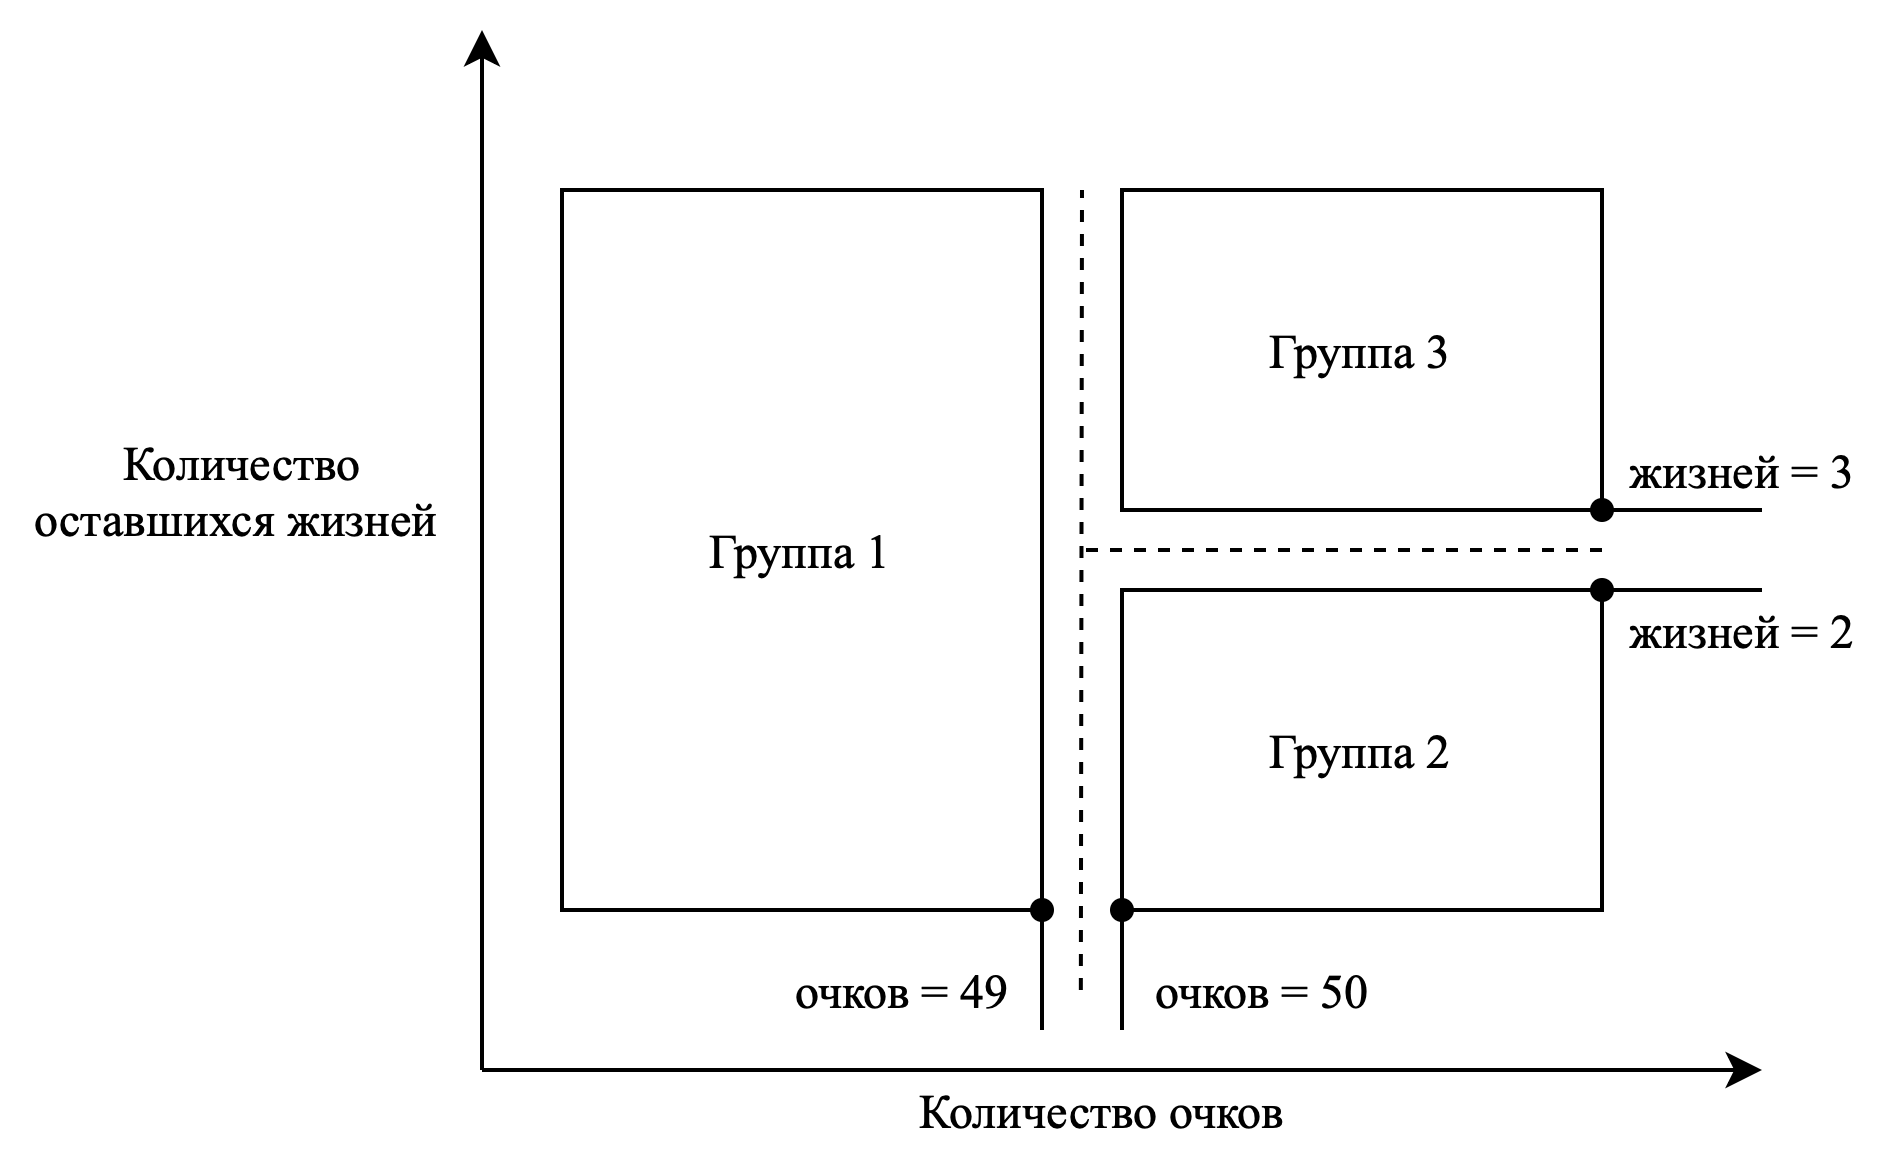
\includegraphics [scale=1.2] {Boundaries_example_TR}
	\caption{Границы групп}
	\label{img:Boundaries_example}
\end{figure}

Тестирующий код представлен в листинге~1.8.

\begin{ListingEnv}[!h]% настройки floating аналогичны окружению figure
	\captiondelim{ } % разделитель идентификатора с номером от наименования
	\caption{Тестирование границ}
	% окружение учитывает пробелы и табуляции и применяет их в сответсвии с настройками
	\begin{lstlisting}[language={Java}]
@Test
void betweenLessAndManyPoints() {
	assertEquals(49+50, pp.totalPoints(49, 5));
	assertEquals(50*3, pp.totalPoints(50, 5));
}

@Test
void betweenLessAndManyLives() {
	assertEquals(500*3, pp.totalPoints(500, 3));
	assertEquals(500+30, pp.totalPoints(500, 2));
}
	\end{lstlisting}
\end{ListingEnv}%



\subsection{Структурное тестирование} 
 
В предыдущих разделах были рассмотренны подходы к разработке тестовых сценариев, которые основанны исключительно на спецификации программы. Далее будут рассмотрены подходы, которые учитывают исходный код программы. Техники, которые используют исходный код программы для разработки тестов, называются техниками \textit{структурного тестирования}.

Основу структурного тестирования составляет \textit{критерий покрытия}. Критерий покрытия тесно связан с понятием \textit{покрытия тестами}. Под~покрытием тестами подразумевается процент всего исходного кода программы, который выполняется в ходе работы тестов.

Приемущества структурного тестирования:

\begin{itemize}
	\item Позволяет разработать тесты исходя только из исходного кода программы. 
	\item Четко определяет критерий полноты тестирования. Это может быть 90~\% (в крайних случаях 100~\%).
\end{itemize}


Далее будут рассмотренны следующие критерии покрытия:

\begin{itemize}
	\item покрытие строк;
	\item покрытие блоков;
	\item покрытие ветвлений;
	\item покрытие условий;
	\item покрытие путей исполнения;
	\item MC/DC покрытие.
\end{itemize}


\subsubsection{Критерий покрытия строк}

Покрытие строк (англ. line coverage)~--- критерий покрытия, основанный на подсчете исполненых в ходе выполнения тестов строк кода. Расчитывается этот критерий как процентное соотношение исполненых в~ходе выполнения тестов строк кода к общему числу строк кода.

\[ \text{покрытие строк} = \frac{\text{количество исполненных строк}}{\text{общее количество строк}}  \times 100 \% \]

Для демострации подсчета этого критерия рассмотрим следующий пример. Программа принимает на вход два числа~-- колличество очков первого игрока и количество очков второго игрока. Программа должна возвращать количество очков победителя. Победителем становится игрок, набравший максимально близкое к 21 количество очков. Если игрок набрал больше очков чем 21, он проигрывает. Если оба игрока проиграли, программа должна вернуть 0. Реализация представлена в листинге~1.9. Тестирующий код представлен в листинге~1.10.

\begin{ListingEnv}[!h]% настройки floating аналогичны окружению figure
	\captiondelim{ } % разделитель идентификатора с номером от наименования
	\caption{Реализация программы Black Jack}
	% окружение учитывает пробелы и табуляции и применяет их в сответсвии с настройками
	\begin{lstlisting}[language={Java}]
public class BlackJack {
	public int play(int left, int right) {
		1.  int ln = left;
		2.  int rn = right;
		3.  if (ln > 21)
		4.    ln = 0;
		5.  if (rn > 21)
		6.    rn = 0;
		7.  if (ln > rn)
		8.    return ln;
		9.  else
		10.   return rn;
	}
}
	\end{lstlisting}
\end{ListingEnv}%

\begin{ListingEnv}[!h]% настройки floating аналогичны окружению figure
	\captiondelim{ } % разделитель идентификатора с номером от наименования
	\caption{Тестирующий код}
	% окружение учитывает пробелы и табуляции и применяет их в сответсвии с настройками
	\begin{lstlisting}[language={Java}]
public class BlackJackTest {
	@Test
	void bothPlayersGoTooHigh() {
		int result = new BlackJack().play(30, 30);
		assertThat(result).isEqualTo(0);
	}
	
	@Test
	void leftPlayerWins() {
		int result = new BlackJack().play(10, 9);
		assertThat(result).isEqualTo(10);
	}
}
	\end{lstlisting}
\end{ListingEnv}%

Первый тест выполняет строки 1-7 и 10. Покрытие этого теста составляет  90~\%. 

\[  \frac{9}{10}  \times 100 \% = 90 \% \]

Не исполненной остается только строка 8. Второй тест её исполяет. Таким образом, покрытие теста \texttt{BlackJackTest} составляет 100~\%

Главной проблемой критерия покрытия строк является то, что этот критерий не всегда отражает реальное покрытие всех возможных сценариев выполнения программы. В листинге~1.11 представлена другая реализация поставленной ранее задачи.

\begin{ListingEnv}[!h]% настройки floating аналогичны окружению figure
	\captiondelim{ } % разделитель идентификатора с номером от наименования
	\caption{Компактная реализация программы Black Jack}
	% окружение учитывает пробелы и табуляции и применяет их в сответсвии с настройками
	\begin{lstlisting}[language={Java}]
public int play(int left, int right) {
	1.  int ln = left;
	2.  int rn = right;
	3.  if (ln > 21) ln = 0;
	4.  if (rn > 21) rn = 0;
	5.  if (ln > rn) return ln;
	6.  else return rn;
}
	\end{lstlisting}
\end{ListingEnv}%

В таком случае покрытие теста \texttt{BlackJackTest.leftPlayerWins} составляет 83~\%. Однако тот же самый тест показыкает покрытие в 60~\% в первой реализации \texttt{BlackJack}. Покрытие строк зависит не только от~тестового сценария и набора входных данных, но и от конкретного стиля написания кода. 


\subsubsection{Критерий покрытия блоков}

Граф потока управления~--- представление всех путей исполнения кода. Он состоит из \textit{базовых блоков, управляющих блоков и рёбер}. Пример графа управления для программы \texttt{BlackJack} из листинга 1.9 представлен на~рис.~1.2. 

\begin{figure}[ht]
	\centering
	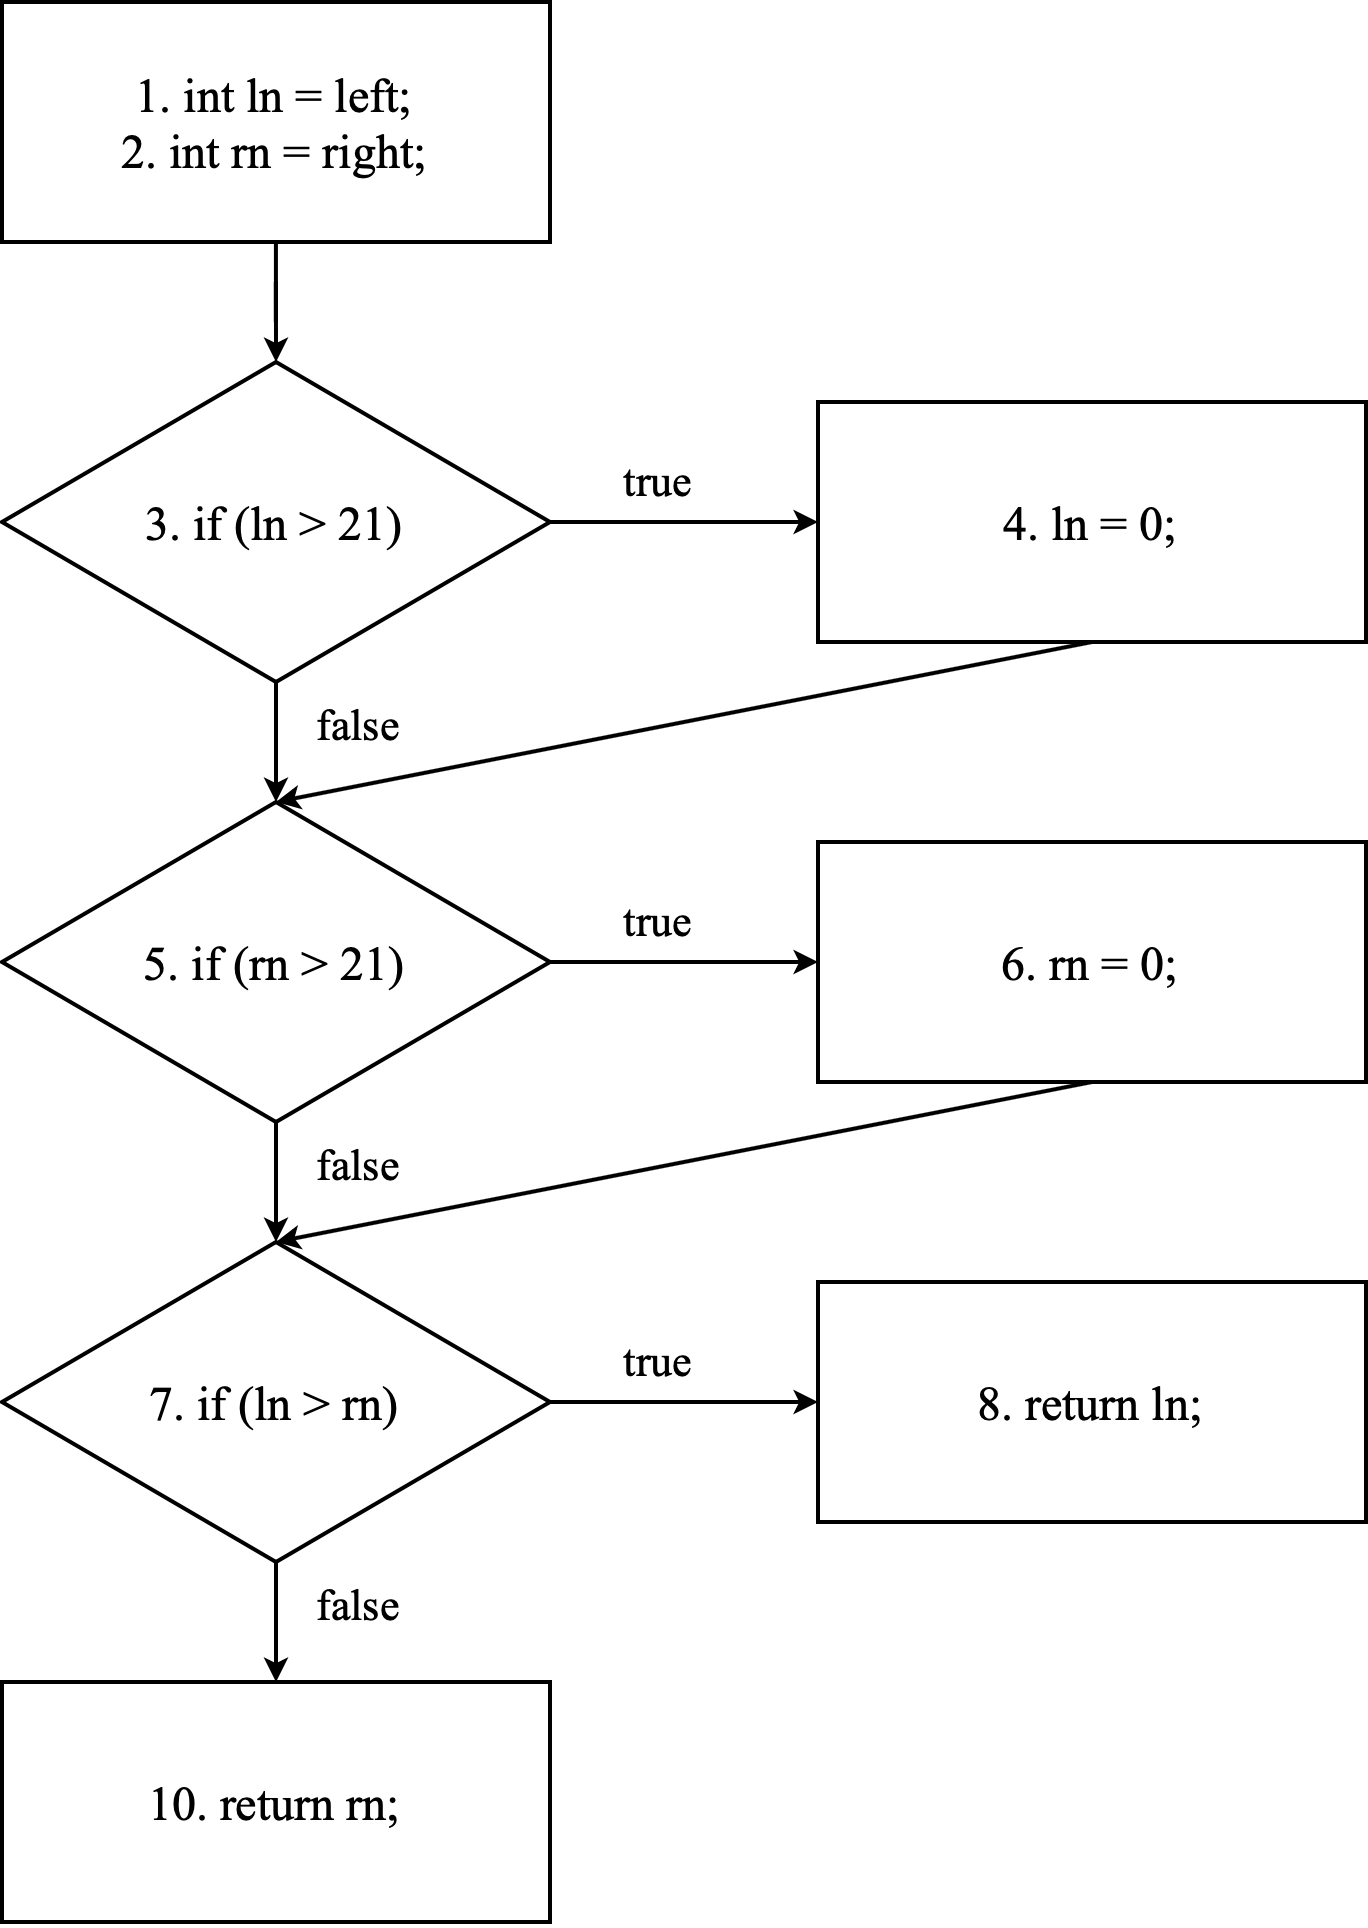
\includegraphics [scale=1.2] {CFG}
	\caption{Граф потока управления для программы \texttt{BlackJack}}
	\label{img:cfg}
\end{figure}

Приемущество графа выполнения состоит в~том, что он практически не~зависит от~языка программирования, на~котором написанна программа. 

Покрытие блоков~--- критерий покрытия, основанный на подсчете соотношения задействованных в ходе выполнения тестов блоков к общему числу блоков в графе потока управления программы.

\[ \text{покрытие блоков} = \frac{\text{количество задействованных блоков}}{\text{общее количество блоков}}  \times 100 \% \]

Критерий покрытия блоков более устойчив к изменениям форматирования исходного кода, чем критерий покрытия строк.


\subsubsection{Критерий покрытия ветвлени}

Покрытие ветвлений~--- критерий покрытия, основанный на подсчете соотношения задействованных в ходе выполнения программы блоков и ребер к общему числу блоков и ребер в графе управления программы. По сути, это расширенный критерий порытия блоков. 


Комбинация из ребра и блока составляет \textit{решение} или \textit{ветвь}. На основе решиний или ветвей и строится критерий покрытия ветвлений.

\[ \text{покрытие ветвлений} = \frac{\text{количество задействованных ветвей}}{\text{общее количество ветвей}}  \times 100 \% \]


На практике критерий покрытия ветвлений оказывается предпочтитель-нее. Он отражает более четкую картину. Например, на графе потока управления в один блок могут приводить несколько ребер. Это означает, что при использовании покрытия блоков, достаточно выполнить блок всего один раз, чтобы достичь 100~\% покрытия. В то время как одно из ребер не будет выполенно. Покрытие ветвлений решает эту проблему.

\subsubsection{Критерий покрытия условий}

Покрытие ветвлений предоставляет два состояния для каждого управляющего блока (условие выполнено или нет). В тех случаях, когда условие внутри управляющего блока состоит из более чем одного логического оператора, покрытия ветвлений недостаточно. 

Например, \texttt{a > 10 \&\& b < 20 \&\& c < 10}. Чтобы достичь 100 \% покрытия по критерию ветвлений, достаточно подобрать два набора входных параметров: (a=20, b=10, c=5)~-- \texttt{true} и (a=5, b=10, c=5)~-- \texttt{false}. Однако, эти наборы вводных данных не покрывают все логические комбинации. Например: (a=20, b=30, c=5)~-- \texttt{false}.

Базовый критерий покрытия условий решает эту проблему. Его суть состоит в трансформации исходного графа выполнения в граф выполнения, который не содержит составных логических условий. 

\[ \text{покрытие условий} = \frac{\text{количество задействованных условий}}{\text{общее количество условий}}  \times 100 \% \]

Одного покрытия условий бывает недостаточно. 100\% покрытие условий не гарантирует 100~\% покрытия всех возможных путей выполнения программы. На практике используется C/DC покрытие (Conditions/Decisions coverage). Оно включает в себя покрытие условий и покрытие ветвлений.

\[ \text{ C/DC} = \frac{P_1 + P_2}{M_1 + M_2} \times 100 \% \]

Где \(P_1\)~--- количество задействованных условий, \(P_2\)~--- количество задействованых ветвей, \(M_1\)~--- общее количество условий, \(M_2\)~---общее количество ветвей.

\subsubsection{Критерий покрытия путей исполнения}

C/DC критерий приводит к большому количеству возможных тестовых сценариев. Это происходит потому, что для разработки тестовых сценариев используются все возможные исходы всех логических условий, а так же всех блоков выполнения.

Критерий покрытия путей исполнения сосредоточен на подсчете уникальных путей, вместо подсчета результатов блоков выполнения и условных блоков. На графе выполнения программы путём является уникальный маршрут из блока A в блок B.

\[ \text{покрытие путей исполнения} = \frac{\text{количество задействованных путей}}{\text{общее количество путей}}  \times 100 \% \]

\subsubsection{MC/DC покрытие}

MC/DC покрытие (Modified C/DC) очень похоже на покрытие путей исполнения. Отличие состоит в том, что MC/DC учитывает не все возможные пути выполнения, а только <<важные>>. В результате общее количество тестов сокращается.

Ключевая идея MC/DC: выполнить каждое условие таким образом, чтобы оно изменило результат программы, независимо от других условий. Рассмотрим пример условного оператора в листинге 1.12.

\begin{ListingEnv}[!h]% настройки floating аналогичны окружению figure
	\captiondelim{ } % разделитель идентификатора с номером от наименования
	\caption{Пример условного оператора}
	% окружение учитывает пробелы и табуляции и применяет их в сответсвии с настройками
	\begin{lstlisting}[language={Java}]
if (!Character.isLetter(str.charAt(i)) 
& (last == 's' | last == 'r')) {
	words++;
}
	\end{lstlisting}
\end{ListingEnv}%

Его можно интерпритировать как \texttt{(A \& (B | C))} следующим образом:

\begin{itemize}
	\item \texttt{A = !Character.isLetter(str.charAt(i))};
	\item \texttt{B = last == 's'};
	\item\texttt{C = last == 'r'}.
\end{itemize}

Чтобы достичь 100~\% покрытия, используя критерий покрытия путей, нужно написать 8 тестовых сценариев (\(2^3\)). MC/DC критерий позволяет сократить число тестовых сценариев до 4. Проблема состоит в том, что бы выбрать из 8 возможных тестовых сценариев необходимые 4. Суть подбора заключается в следующем:  каждый следующий тестовый сценарий должен изменять результат работы программы (по сравнению с~предыдущим тестовым сценарием), при этом набор входных параметров должен отличаться не более, чем на один параметр.  Алгоритм подбора тестовых данных для программы из листинга~1.11: 

\begin{itemize}
	\item \texttt{(A = true, B = false, C = true) = true}. Изменяем параметр C.
	\item \texttt{(A = true, B = false, C = false) = false}. Изменяем параметр B.
	\item \texttt{(A = true, B = true, C = false) = true}. Изменяем параметр A.
	\item \texttt{(A = false, B = true, C = false) = false}.
\end{itemize}

Приемуществом MC/DC критерия является меньшее количество наборов тестовых данных (N + 1, N - количество входных параметров) по сравнению с критерием покрытия путей (\(2^N\), N - количество входных параметров).


\subsubsection{Выбор критерия порытия}

Приведенные критерии покрытия имеют разные свойства. Некоторые из них просты и интуитивны. Другие покрывают максимально возможное количество путей исполнения программы, но~обладают сложностью в~реализации. На рис~1.3 показанно отношение критериев с точки зрения полноты покрытия.

\begin{figure}[ht]
	\centering
	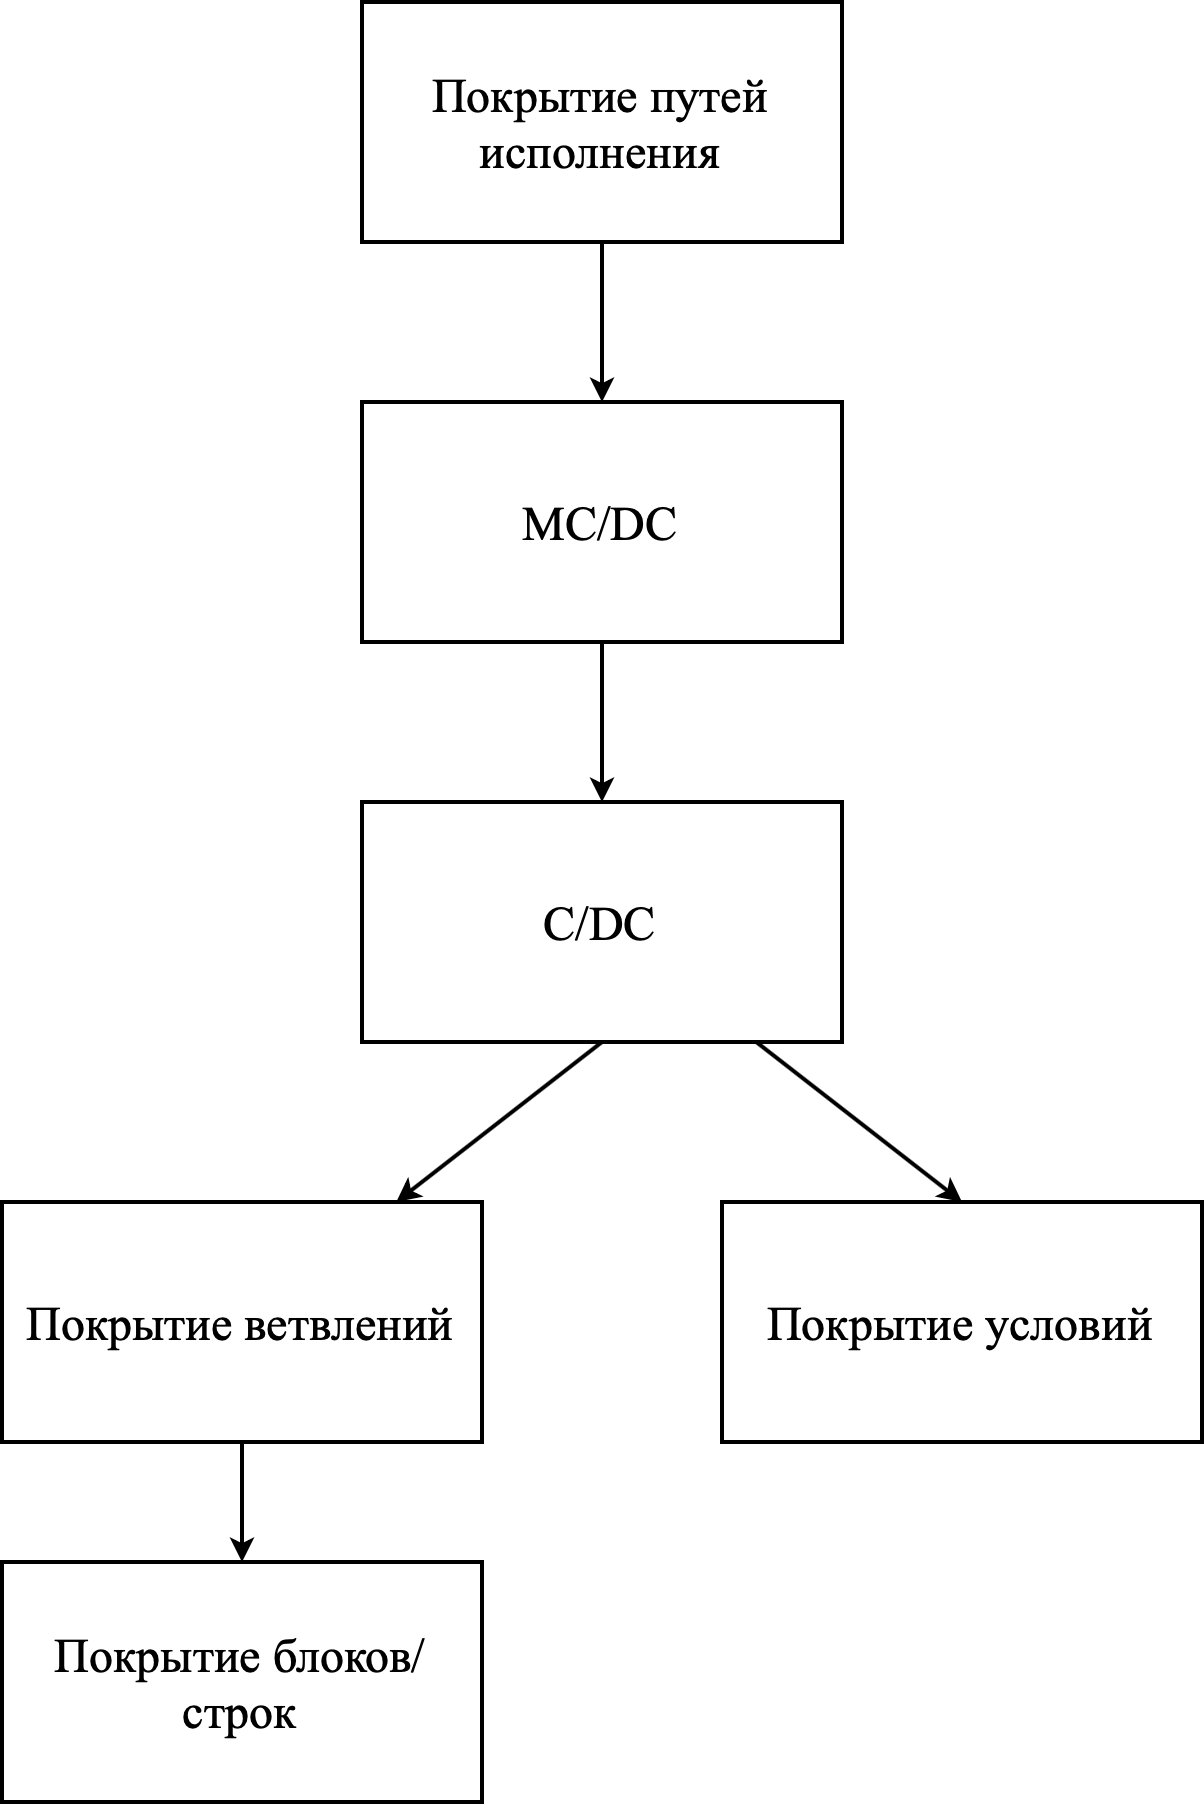
\includegraphics [scale=1.2] {Coverage_criteria_TR}
	\caption{Соотношение критериев покрытия}
	\label{img:Cov_criteria}
\end{figure}

Например, 100~\% покрытие ветвлений автоматически означает 100~\% покрытия строк кода. Но 100~\% покрытия MC/DC не означает 100~\% покрытия путей исполнения. 

На практике критерий покрытия строк кода является самым быстрым и простым. Если требуется более делальное покрытие, выбирается MC/DC. 

В больших программах сложно добиться 100~\% покрытия. Часто это не выгодно с точки зрения затраченных человеческих ресурсов.  Рекомендованный порог покрытия 90~\% [5].

Важно отметить, что структурное тестирование, не зависимо от выбранного критерия покрытия, не способно полностью заменить тестирование на основе спецификации. Структурное тестирование хорошо дополняет тестирование на основе спецификации.

\subsection{Тестирование на основе модели} 
 

Модель~--- способ формализации работы тестируемой системы. Модель используется для анализа и тестирования программного обеспечения. Далее будут рассмотрены два вида моделей: \textit{таблицы решений} и \textit{конечные автоматы}.


\subsubsection{Таблицы решений}

Таблица решений~--- таблица, состоящая из \textit{условий} и \textit{действий}, которые выполняет программа при указанных условиях.

Таблицы решений используются для моделирования того, как комбинация входных параметров приводит к определённому результату выполнения программы.

Пример таблицы решений представлен в~табл.~\ref{decision_table}.

\begin{table} [h!tbp]
	\centering
	\changecaptionwidth\captionwidth{16.37cm}
	\caption{Пример таблицы решений}\label{decision_table}%
	\begin{tabular}{| p{2.5cm} | p{2.9cm} | p{2.1cm} | p{2.1cm} | p{2.1cm} | p{2.1cm} | } 				  \hline
									 					 &					     &	\multicolumn{4}{ | c | }{\textbf{Варианты}}					\\ \hline
	\multirow{2}{*}{\textit{Условия}}  	 & <Условие1>   &  T 			   &  T 			  &  F 				  &  F			     \\  \cline{2-6}
								 	 					  & <Условие2>   &  T	 		   &  F 			  &  T 			     &  F			     \\ \hline
		\textit{Действие}						& <Действие>	& значение1	& значение2 & значение3 & значение4	 \\ \hline	
	\end{tabular}
\end{table}	

Таблица содержит все комбинации условий (\(2^N\)). На практике, условия, не влияющие на результат, помечаются как dc (don't care) и не участвуют в~комбинировании входных данных.
 
Существует несколько стратегий написания тестовых сценариев, основанных на таблице решений:

\begin{itemize}
	\item Все варианты, представленные в таблице. Каждая колонка в~таблице~--- отдельный набор тестовых сценариев.
	\item Все возможные варианты. Каждый набор входных данных~--- уникальная комбинация. Количество таких комбинаций \(2^N\). На~практике это почти недостижимый способ разработки тестовых сценариев.
	\item Учитывание уникальных действий. Каждый тестовый сценарий приводит к уникальному действию.
	\item Каждое условие является истиным и ложным. Каждое условие в~таблице решений должно принять оба своих состояния: \texttt{true}  и~\texttt{false}. Чаще всего это приводит к двум наборам входных данных: все условия истинны и~все условия ложны.
	\item MC/DC. Применение техники MC/DC к таблице решений.
\end{itemize}

Для написания сценариев тестирования, основанных на таблице решений, часто используются параметризованные тесты JUnit 5.

\subsubsection{Конечные автоматы}

Модель конечных автоматов описывает \textit{состояния} системы и \textit{переходы} между ними. Состояние отражает конкретное место в коде в момент выподнения.  Переход~--- действие, которое переводит систему из одного состояния в другое. Помимо состояний и переходов, конечный автомат имеет \textit{начальное состояние} и \textit{события}. Начальное состояние~--- состояние, с~которого начинается работа системы. События~--- описание того, что происходит в процессе перехода. 

Конечные автоматы представляются в виде UML диаграммы. Пример конечного автомата представлен на рис.~\ref{img:state_machine}

\begin{figure}[ht]
	\centering
	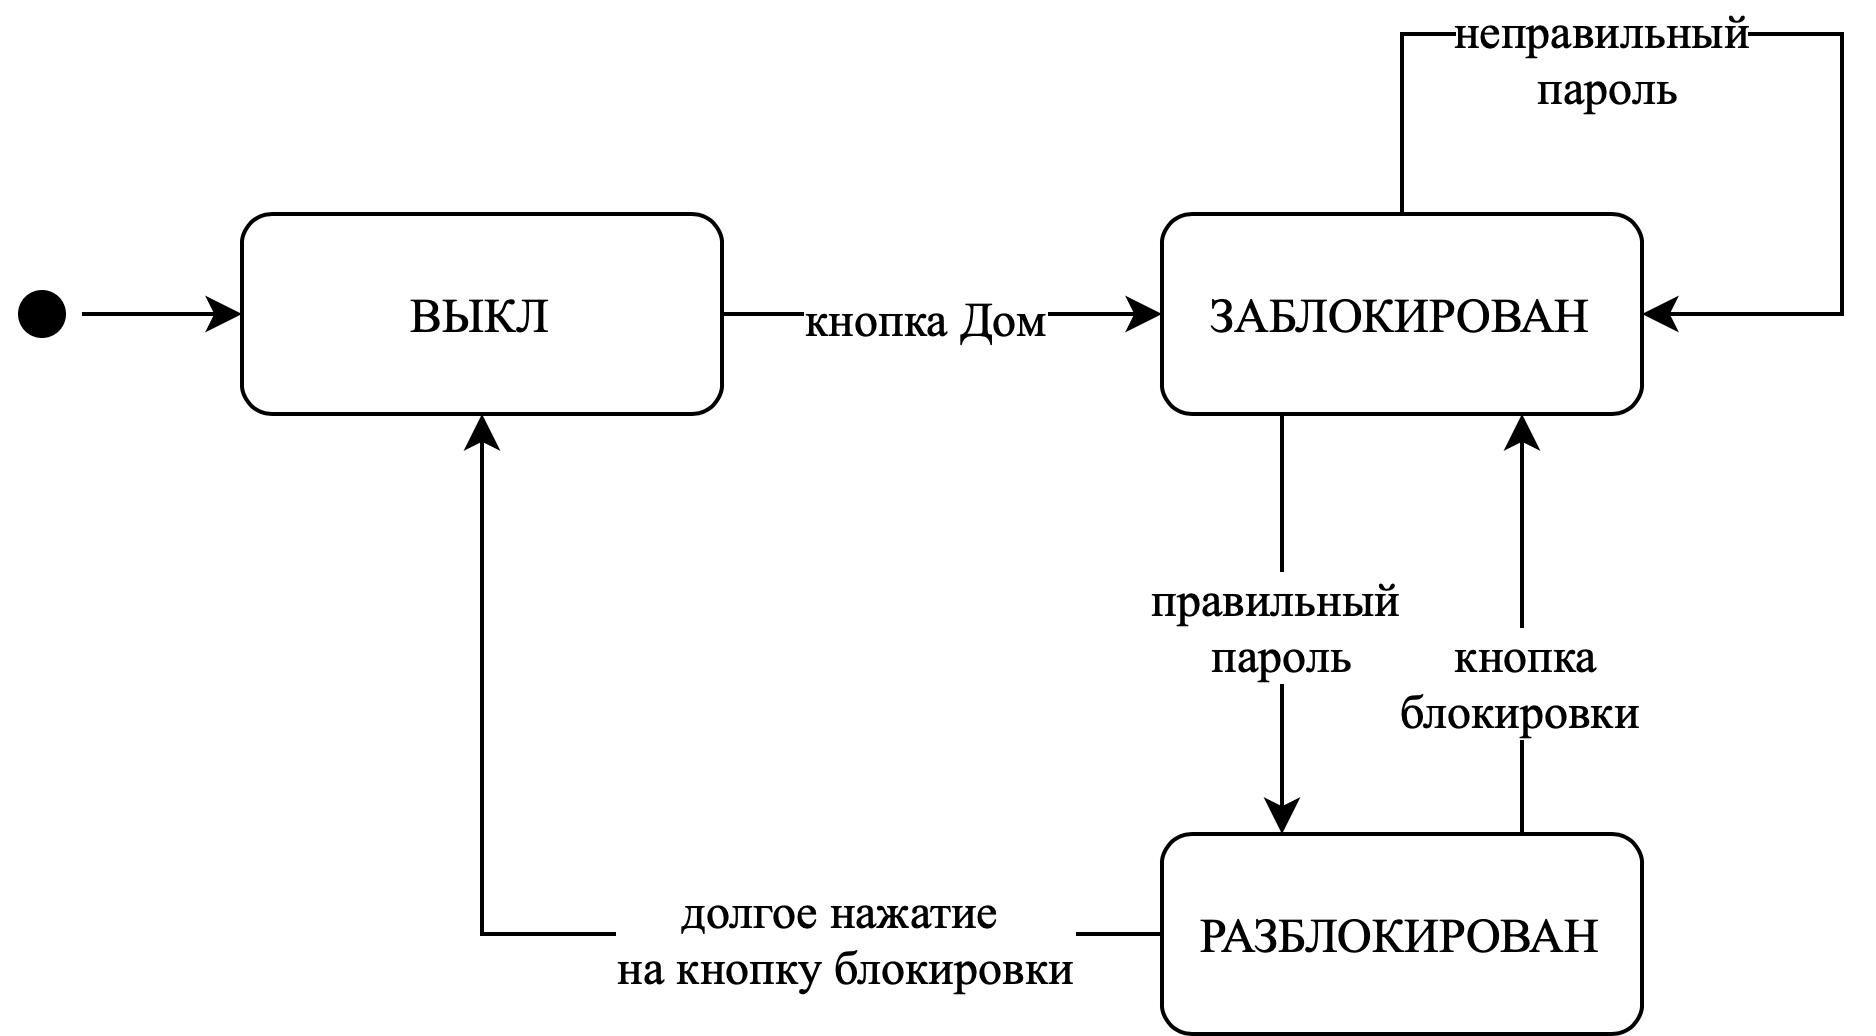
\includegraphics [scale=1.2] {State_machine_TR}
	\caption{Конечный автомат главного экрана телефона}
	\label{img:state_machine}
\end{figure}


Для разработки тестовых сценариев на основе конечного автомата, необходимо преобразовать конечный автомат в \textit{дерево переходов}. Пример дерева переходов представлени на рис.~\ref{img:transition_tree}

\begin{figure}[ht]
	\centering
	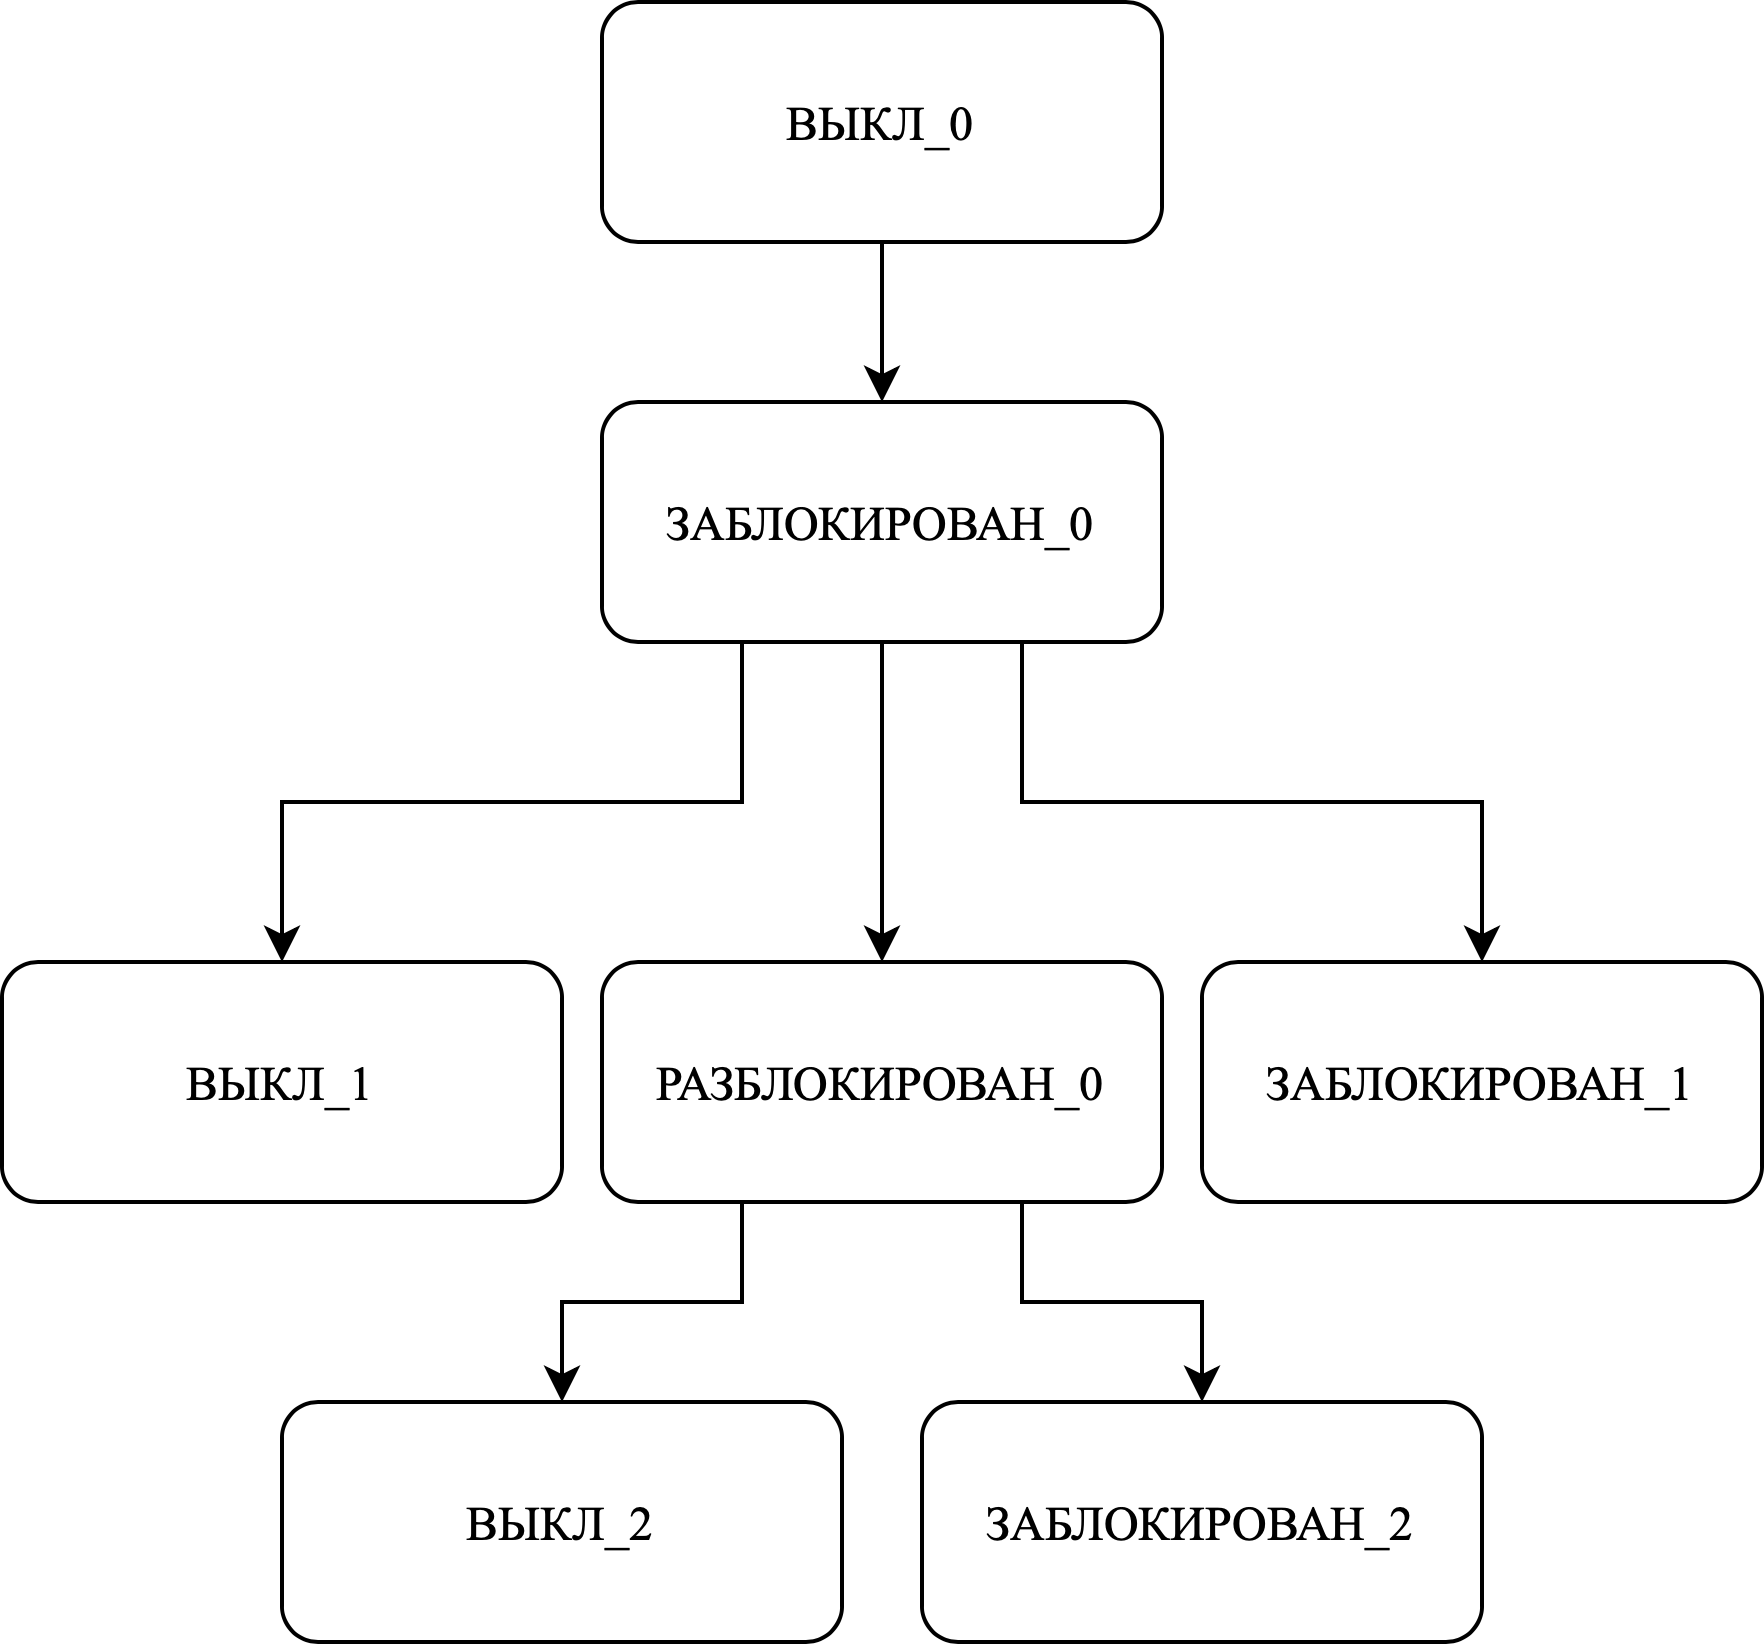
\includegraphics [scale=1.2] {Transition_tree_TR}
	\caption{Дерево переходов главного экрана телефона}
	\label{img:transition_tree}
\end{figure}

Из дерева переходов можно разработать набор тестовых сценариев. Техника подбора тестовых сценариев проста: нужно посетить все листья дерева переходов. Такой подход близок к структурному тестированию с~критерием покрытия путей исполнения.

Описанный подход позволяет формализовать разработку тестов. Однако, для разработки понятных и поддерживаемых тестов на основе конечного автомата часто требуются дополнительные усилия. Например, введение нового уровня абстракции в кодовую базу тестов (интроспецкия состояний и переход из одного состояния в другое). 


\subsection{Тестирование на основе контракта} 
 
\subsubsection{Самотестируемые программы}

Программа, которая тестирует свое поведение в ходе исполнения, называется самотестируемой. До настоящего момента были рассмотренны подходы к тестированию программного обеспечения, которые подразумевают написание отдельного кода с тестами. Самотестируемые программы исключают написание специального кода для тестов. Они содержат тесты внутри себя.  Далее будут рассмотренны способы реализации самотестируемых программ.

\subsubsection{Утверждения}

Самый простой способ проверить состояние программы на~соответствие какому-либо условию~--- утверждения (assertions). Пример программы с утверждениями представлени в листинге~1.13.

\begin{ListingEnv}[!h]% настройки floating аналогичны окружению figure
	\captiondelim{ } % разделитель идентификатора с номером от наименования
	\caption{Пример утверждения}
	% окружение учитывает пробелы и табуляции и применяет их в сответсвии с настройками
	\begin{lstlisting}[language={Java}]
public class MyStack {
	public Element pop() {
		assert count() > 0 : "The stack does not have any elements to pop";
		
		// ... actual method body ...
		
		assert count() == oldCount - 1 : "Size of stack did not decrease by one";
	}
}
	\end{lstlisting}
\end{ListingEnv}%


Утверждения играют роль \textit{оракулов}. Они информируют программиста в случае, если программа работает некорректно. 

Стоит отметить, что утверждения не заменяют модульное тестирование. 


\subsubsection{Предусловия и постусловия}	

Понятия предусловия и постусловия определяются в \textit{логике Хоара}, а~именно \textit{тройками Хоара}~[6]. Тройка Хоара выглядит следующим образом: \[\{P\} \space C \space \{Q\}\]

где \textit{P} и \textit{Q} являются утверждениями, а \textit{C}~--- командой (выражение, метод). \textit{P}~--- предусловие, \textit{Q}~--- постусловие. Можно утверждать, что если выполнено предусловие \textit{P}, то команда \textit{C} будет исполнена. Если предусловие \textit{P} не выполнено, то команда \textit{C} не может быть выполнена. Если команда \textit{C} выполнена, то гарантируется соблюдение постусловия \textit{Q}.

Пример программы с предусловиями и постусловиями представлен в~листинге~1.14.

\begin{ListingEnv}[!h]% настройки floating аналогичны окружению figure
	\captiondelim{ } % разделитель идентификатора с номером от наименования
	\caption{Программа с постусловиями и предусловиями}
	% окружение учитывает пробелы и табуляции и применяет их в сответсвии с настройками
	\begin{lstlisting}[language={Java}]
public class FavoriteBooks {
	// ...
	
	public void merge(List<Book> books) {
		assert books != null : "The list of books is null";
		assert favorites != null : "The favorites list is null";
		
		List<Book> newBooks = books.removeAll(favorites);
		
		if (!newBooks.isEmpty()) {
			favorites.addAll(newBooks);
			pushNotification.booksAdded(newBooks);
		}
		
		assert favorites.containsAll(books) : "Not all books were added to favorites";
	}
}
	\end{lstlisting}
\end{ListingEnv}%

Важное замечание: если не было выполнено предусловие, то метод не~может гарантировать соблюдение постусловия.

\subsubsection{Инварианты}	

Инвариант программы~--- условие, которое выполняется на~протяжении всего времени жизни программы. Отличие инварианта от~предусловия или постусловия в том, что предусловие выполняется только до~выполнения метода, а постусловие только после. Инвариант выполняется всегда.

Для проверки инварианта, как правило, создается проверяющий метод. Пример проверяющего метода представлен в листинге~1.15. Он проверяет, что дочерние элементы двоичного дерева всегда содержат указатель на~родительский элемент.

\begin{ListingEnv}[!h]% настройки floating аналогичны окружению figure
	\captiondelim{ } % разделитель идентификатора с номером от наименования
	\caption{Пример проверяющего метода}
	% окружение учитывает пробелы и табуляции и применяет их в сответсвии с настройками
	\begin{lstlisting}[language={Java}]
public void checkRep(BinaryTree tree) {
	BinaryTree left = tree.getLeft();
	BinaryTree right = tree.getRight();
	
	assert (left == null || left.getParent() == tree) &&
	(right == null || right.getParent() == tree) :
	"A child does not point to the correct parent";
	
	if (left != null) {
		checkRep(left);
	}
	if (right != null) {
		checkRep(right);
	}
}
	\end{lstlisting}
\end{ListingEnv}%


Инварианты могут быть не только на уровне метода. В объектно-ориентированных языках часто встречаются \textit{инварианты классов}. Инвариант класса~--- условие, которое выполняется на протяжении всей жизни экземпляра класса. Такие инварианты проверяются в конструкторе, вначале и конце всех публичных методов.

\subsubsection{Дизайн по контракту}	

Дизайн по контракту~--- дизайн системы, которая соблюдает предусловия, постусловия и инварианты. В клиент-серверных приложениях дизайн по контракту играет значимую роль. Для успешной коммуникации клиента с сервером, клиент должен соблюдать предусловия сервера. А~сервер гарантирует соблюдение постусловий и инвариантов. На практике контрактом является интерфейс. Диаграмма на рис.~\ref{img:design_by_contract} иллюстрирует контракт, обьявленный интерфейсом и его имплементацию. 

\begin{figure}[ht]
	\centering
	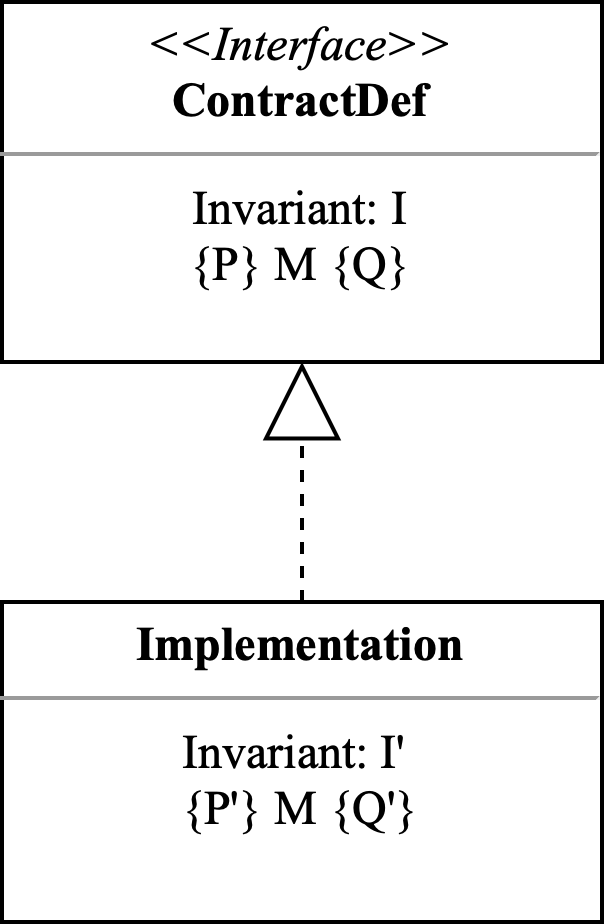
\includegraphics [scale=1.2] {Design_by_contract_TR}
	\caption{Контракт и его реализация}
	\label{img:design_by_contract}
\end{figure}


\subsection{Тестирование свойств} 

Тестирование свойств (Property-based testing)~--- герерация псевдо-случайных наборов входных данных с целью поиска ошибок в программе. Первая реализация этой идеи называется \textit{QuickCheck}~[7], написанная для языка Haskell. Сейчас многие языки имеют аналоги данного инструмена. Тестирование свойств в Java производится с помощью библиотеки \textit{jqwik}~[8].

Для того, что бы использовать \textit{jqwik}, необходимо определить метод и пометить его аннотацией \texttt{@Property} (аналог аннотации \texttt{@Test}). После этого нужно добавить в аннотированный метод параметры и пометить их аннотацией \texttt{@ForAll} (есть множесто других аннотаций). 

Для примера определим свойство конкатенации двух строк: для любых двух строк результат их конкатенации должен иметь длинну, равную сумме длин исходных строк. Пример тестирования свойства с помощью jqwik представлен в листинге~1.16.

\begin{ListingEnv}[!h]% настройки floating аналогичны окружению figure
	\captiondelim{ } % разделитель идентификатора с номером от наименования
	\caption{Тестирование свойста конкатенации двух строк}
	% окружение учитывает пробелы и табуляции и применяет их в сответсвии с настройками
	\begin{lstlisting}[language={Java}]
public class PropertyTest {
	
	@Property
	void concatenationLength(@ForAll String s1, @ForAll String s2) {
		String s3 = s1 + s2;
		
		Assertions.assertEquals(s1.length() + s2.length(), s3.length());
	}
}
	\end{lstlisting}
\end{ListingEnv}%

Jqwik сгенерирует множество псевдо-случайных входных данных (s1 и s2) и проверит выполение утверждения.
